\newcommand{\assignmentDate}{November 25th, 2019}

% Add title
%Institute
\begin{tabular*}{\hsize}{l@{\extracolsep{\fill}} r}
	\textsc{Technical University of Berlin}		 \hfill&								 	\\
	Faculty II - Mathematics and Natural Sciences\hfill&									\\
	Institute of Mathematics 					 \hfill&									\\
	Dr. D. Peschka, A. Selahi 		 			 \hfill&									\\
\end{tabular*}

% Title
\begin{center}
	\textbf{\Large{\courseName}}\\
	\vspace{7pt}
	\large{Homework \currentAssignment}\\
	\smallskip
	\normalsize{Submitted on \assignmentDate}
\end{center}

% Group table
\begin{center}
	\vspace{-8pt}
	\begin{tabular}{l c r}
		by \textbf{\groupNumber}		    &	 			  &		 								\\
		\hline
		\texttt{Kagan Atci} 			    & \texttt{338131} & \texttt{Physical Engineering, M.Sc.}\\
		\texttt{Navneet Singh }		 	    & \texttt{380443} & \texttt{Scientific Computing, M.Sc.}\\ 
		\texttt{Daniel V. Herrmannsdoerfer} & \texttt{412543} & \texttt{Scientific Computing, M.Sc.}\\ 
		\hline
	\end{tabular}
\end{center}

% EXERCISE 1
% --------------------------------------------------------------------------------------------------------------------
\newcommand{\Lhalf}{\frac{L}{2}}
\addExercise{1}{Ex1}
Given is the Poisson problem on general domains $\bar{\Omega} \subset [0, L]^2 \subset \mathbb{R}^2$ for given functions $f, g \colon \mathbb{R}^2 \rightarrow \mathbb{R}^2$, considering
%
\begin{equation}
	\label{eq:problem}
	-\Delta u = f \text{ in } \Omega,\; u = g \text{ on } \partial \Omega \text{.}
\end{equation}
% ----------------
\addSubExercise{a}
The considered domain is
\begin{equation}
	\label{eq:domain1}
	\bar{\Omega} = \{(x,y) \in (0,L)^2 \colon \left(x-\Lhalf \right)^2 + \left(y - \Lhalf \right)^2 \leq 1 \}
\end{equation}

with  $L =2.2$ and built-up in a $\mathbb{R}^N \times \mathbb{R}^N$ environment, where $N = 256$.
As illustrated in \FIG{a05ex01grid}, the points contained in $\Omega_h$ have all direct neighbors in $\bar{\Omega}_h$, where points on $\Gamma_h$ having neighbors outside of $\Omega$.
For the algorithm, please refer to \textit{Boundary Allocation} section in online submitted \texttt{a05ex01\_get\_laplace.m} file.

%
% ----------------
\addSubExercise{b}
Please refer to '\textit{Boundary Allocation}' section in online submitted \texttt{a05ex01\_get\_ laplace.m} file.

%
% ----------------
\addSubExercise{c}
Please refer to '\textit{Differentiation Matrix}' section in online submitted \texttt{a05ex01\_get\_ laplace.m} file.

%
% ----------------
\addSubExercise{d}
The problem from \EQ{problem} and \EQ{domain1} was solved numerically using $256 \times 256$ points with $f = 1$ and $g = 0$.
The solution is plotted in \FIG{a05ex01Laplace256}.
%
\vspace*{\FigUpperVSpace}
\begin{figure}[H]
	\centering
	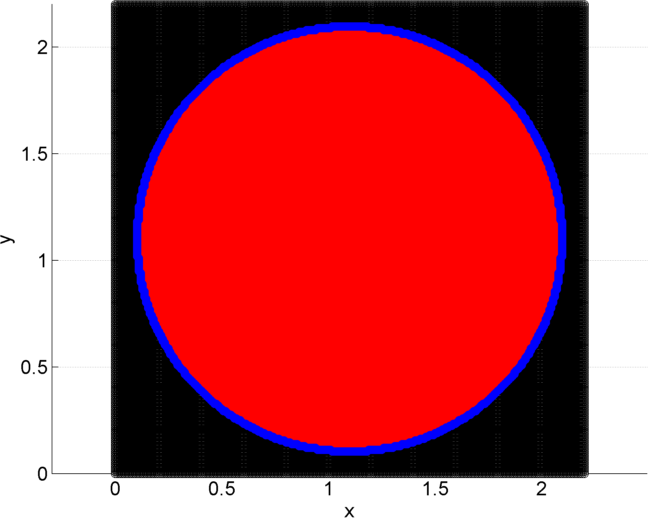
\includegraphics[width=0.68\textwidth]{a05ex01grid.png} 
	\caption{The domain and sub-domain in 2D. The red area represents $\Omega_h$ and the blue circle $\Gamma_h$, which in combination makes the sub-domain $\bar{\Omega_h}$.
			 The black area is the part of the domain that is not included into further calculations.
			 The dot-wise plot is due to the high amount of grid points not recognizable.}
	\label{fig:a05ex01grid}
\end{figure}
%
\vspace*{\FigUpperVSpace}
%
\begin{figure}[H]
	\centering
	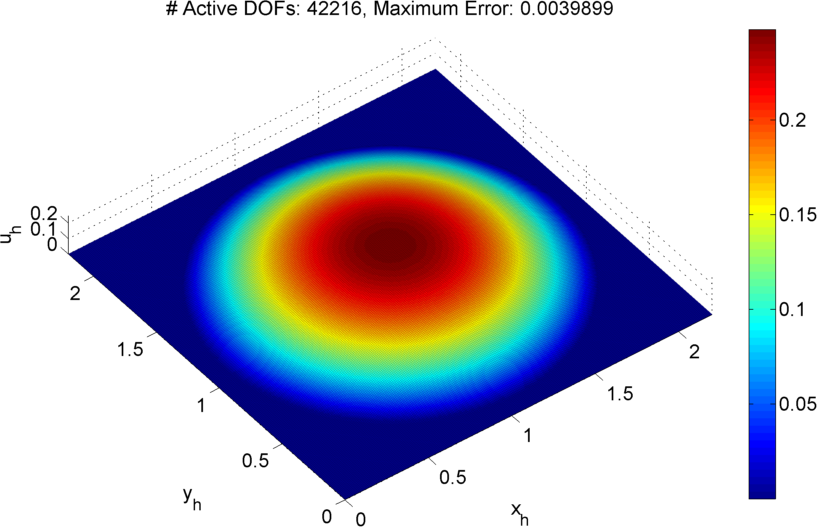
\includegraphics[width=0.9\textwidth]{a05ex01Laplace256.png} 
	\caption{Solution of the \EQ{domain1} with $N = 256$.
			 The magnitude of the U values are labeled with the color bar.
			 Number of active DOFs (also the length of the $L_h$ matrix) and the maximum error between the analytical and the numerical solution is given in the figure title.}
	\label{fig:a05ex01Laplace256}
\end{figure}

%
% ----------------
\addSubExercise{e}
In this sub-exercise, \EQ{problem} and \EQ{domain1} with the previously mentioned boundary conditions were successively solved for $2^N$ points, with $N \in [2,9] \subset \mathbb{N}$.
The error between the analytical and numerical solution, calculated in the form of maximum maximum norm $|| R_h u - u_h||_{\infty , h}$, is displayed in \FIG{a05ex01error}.
%
\vspace*{\FigUpperVSpace}
%
\begin{figure}[H]
	\centering
	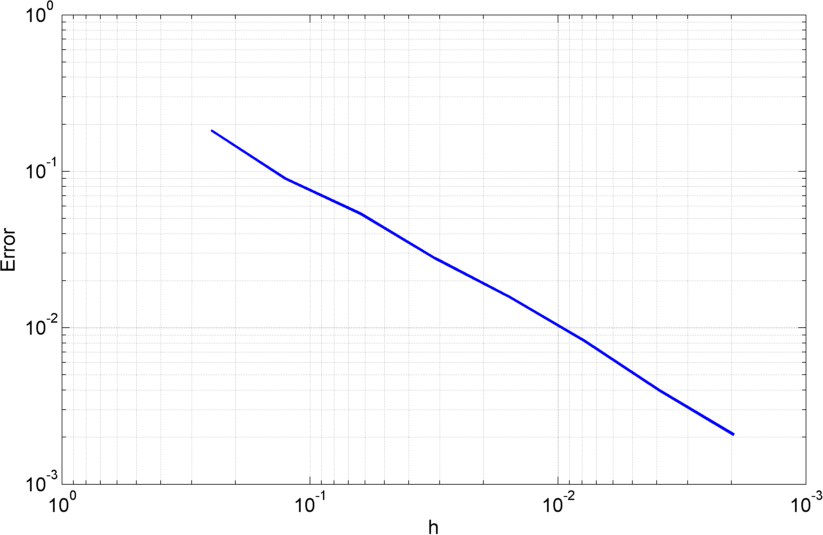
\includegraphics[width=\textwidth]{a05ex01error.png} 
	\caption{Logarithmic diagram of $|| R_h u - u_h||_{\infty , h}$.
			 The direction of the x-axis was flipped, so that $h$ is decreasing towards right the right hand side.
			 Hence, a more comfortable overview can be attained.}
	\label{fig:a05ex01error}
\end{figure}
The order of the convergence is obtained writing the convergence in the form of monomial equation $Error = a \cdot h ^k$, with $a$ the proportion factor, and $k$ the order of the convergence.
Taking the logarithmic line linear, the slope of the line $k$ yields
\begin{equation}
	k = \frac{\log{(Error(h_9) / Error(h_2)})}{\log{(h_9 / h_2)}}\approx 0.92282 \text{ .}
\end{equation}
%
% ----------------
\addSubExercise{f}
Considering
\begin{align}
	\nonumber
	\bar{\Omega} = \{(x,y) \in (0,L)^2 \colon &(x - L/12) &-& \;&0.05 \cos(30 \cdot y / L) 			&\geq 0& \; \land \\
	\nonumber
											  &(x - L/1.1) &-& \;&0.1\cos(30 \cdot y / L) 			&\leq 0& \; \land \\
	\nonumber
											  &(y - L/1.09) &-& \; &0.1\sin(10 \cdot \pi \cdot x / L) &\leq 0& \; \land \\
	\nonumber
											  &(y - L/12) &-& \; &0.1\sin(10 \cdot \pi \cdot x / L) 	&\geq 0& \; \land \\
	\label{eq:domain2}
											  &0.8(x-L/2)^2 &+& \; &1.3(y-L/2)^2  				  	&\geq 0& \} \text{,}
\end{align}
the layout of the sub-domain is illustrated in \FIG{a05ex01domain2}.
The outer boundaries of the sub-domain were modeled with sine functions, as the inner boundary was shaped using an elliptic formulation.\\
%
\vspace*{\FigUpperVSpace}
\begin{figure}[H]
	\centering
	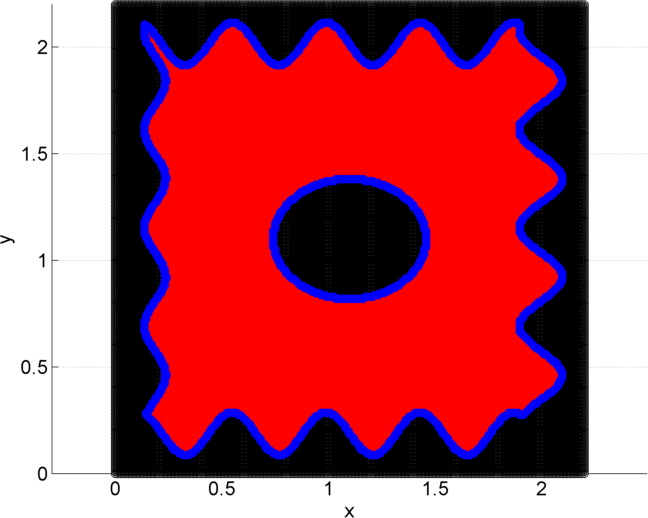
\includegraphics[width=0.68\textwidth]{a05ex01domain2.png} 
	\caption{The layout of the sub-domain of \EQ{domain2}. The definitions of the edges are corresponding in following sequence: First line for left border, Second line for right  border, Third line for upper border, fourth line for lower border, fifth line for the inner elliptic border.}
	\label{fig:a05ex01domain2}
\end{figure}
%
Two types of problems are to be considered for this topology:
\begin{align}
	\label{eq:problem1}
	&f = 1, \;    	 & g = & \;0 \\
	\label{eq:problem2}
	&f = 5x + 3y, \; & g = & \; 0.2 \cdot \sin(6\cdot \pi \cdot x/L) \cdot \sin(6 \cdot \pi \cdot y) + 0.5 \cdot \sin(2\cdot x/L)
\end{align}
The former problem is chosen exactly same in \textbf{d)} for checking the quality of the solution, while the latter problem refers more complex boundary conditions.
The surface plots of the solutions are displayed in \FIG{a05ex01f}.
%
\begin{figure}[H]
\vspace*{\FigUpperVSpace}
\def\MeshFigWidth{210pt}
	\begin{subfigure}[b]{0.5\hsize}
		\centering
		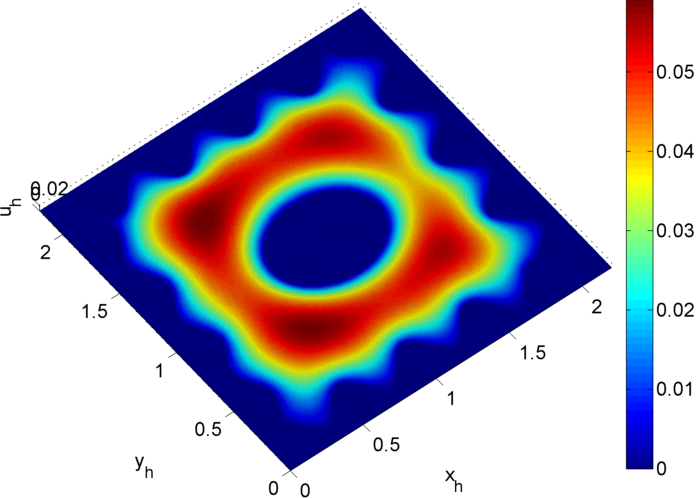
\includegraphics[width=\MeshFigWidth]{a05ex01domain2bound1.png} 
		\caption{First Problem}
		\label{fig:a05ex01domain2bound1}
	\end{subfigure}
	\begin{subfigure}[b]{0.5\hsize}
		\centering
		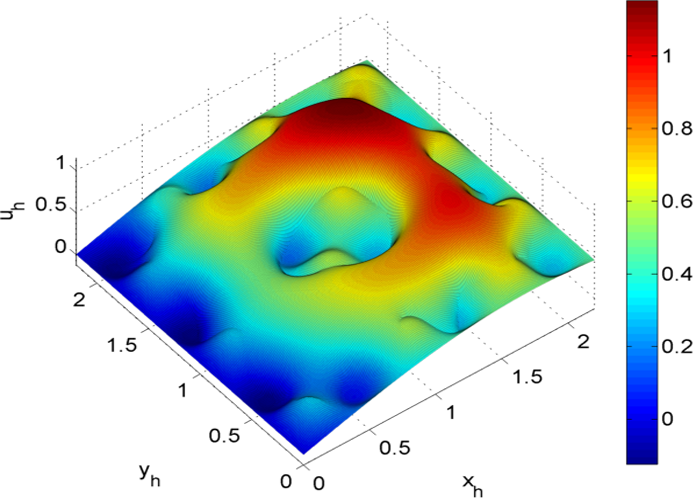
\includegraphics[width=\MeshFigWidth]{a05ex01domain2bound2.png} 
		\caption{Second Problem}
		\label{fig:a05ex01domain2bound2}
	\end{subfigure}
	\caption{Numerical solutions of the above stated problems, where the first problem refers to \EQ{problem1} and second problem to \EQ{problem2}.}
	\label{fig:a05ex01f}
\end{figure}

%
% EXERCISE 2
% --------------------------------------------------------------------------------------------------------------------
\addExercise{2}{Ex2}
%
% ----------------
\addSubExercise{a}
a)

For type i) a solvability condition is required if $\alpha_i=c=0$, since in this case the problem coincides with a von Neumann condition which we know has a non- invertible matrix. As soon as an alpha component is added, the Robin condition is well conditioned, as it is a linear combination of the von Neumann condition and the well conditioned Dirichlet boundary condition.

for ii) we need a boundary condition in any case

b)
Please refer to the program a05e02solvePDE.py to see an implementation of the BVP. Analogously as with the symmetric difference stencil for the von Neumann boundary seen in class, we have chosen to use a symmetric difference stencil here too, since it leads to a better convergernce rate than asymmetric stencils $D^+$ or $D^-$
The 

%
% ----------------
\addSubExercise{b}

%
% ----------------
\addSubExercise{c}

%
% EXERCISE 3
% --------------------------------------------------------------------------------------------------------------------
\addExercise{3}{Ex3}
%
% ----------------
\addSubExercise{a}
The discrete maximum principle states that if the operator is positive for every $x_0$, than the maximum must be on the boundary. Substituting the operator in the inequality, we have:
\begin{gather}
    \Delta_h u_h \ge 0 \nonumber\\
    -8 u(x_0) + \sum_{n=1}^{8} u(x_n) \ge 0 \nonumber\\
    u(x_0) \le  \frac{1}{8} \sum_{n=1}^{8} u(x_n)
    \label{e3eq1}
\end{gather}

Where $x_n$ are the neighboring points of $x_0$. By the \EQ{e3eq1} we know that $x_0$ must be less or equal than the average of the points on its neighborhood.

This implies that for every point $x_0$ in the domain i) either at least one neighbor $x_n$ is larger than $x_0$, or ii)  all neighbors are equal to $x_0$. Therefore the maximum of the function must lay on the boundary of the domain, since it is the only location where it could have a larger neighbor (outside the boundary) and still be the maximum of the domain.
%
% ----------------
\addSubExercise{b}

%
% ----------------
\addSubExercise{c}
%
% ----------------
\addSubExercise{d}